 \documentclass[11pt]{exam}

\usepackage{amssymb, amsmath, amsthm, mathrsfs, multicol, graphicx}
\usepackage{tikz}

 \def\d{\displaystyle}
\def\?{\reflectbox{?}}
\def\b#1{\mathbf{#1}}
\def\f#1{\mathfrak #1}
\def\c#1{\mathcal #1}
\def\s#1{\mathscr #1}
\def\r#1{\mathrm{#1}}
\def\N{\mathbb N}
\def\Z{\mathbb Z}
\def\Q{\mathbb Q}
\def\R{\mathbb R}
\def\C{\mathbb C}
\def\F{\mathbb F}
\def\A{\mathbb A}
\def\X{\mathbb X}
\def\E{\mathbb E}
\def\O{\mathbb O}
\def\U{\mathcal U}
\def\pow{\mathcal P}
\def\inv{^{-1}}
\def\nrml{\triangleleft}
\def\st{:}
\def\~{\widetilde}
\def\rem{\mathcal R}
\def\sigalg{$\sigma$-algebra }
\def\Gal{\mbox{Gal}}
\def\iff{\leftrightarrow}
\def\Iff{\Leftrightarrow}
\def\land{\wedge}
\def\And{\bigwedge}
\def\AAnd{\d\bigwedge\mkern-18mu\bigwedge}
\def\Vee{\bigvee}
\def\VVee{\d\Vee\mkern-18mu\Vee}
\def\imp{\rightarrow}
\def\Imp{\Rightarrow}
\def\Fi{\Leftarrow}

%\def\={\equiv}
\def\var{\mbox{var}}
\def\mod{\mbox{Mod}}
\def\Th{\mbox{Th}}
\def\sat{\mbox{Sat}}
\def\con{\mbox{Con}}
\def\bmodels{=\joinrel\mathrel|}
\def\iffmodels{\bmodels\models}
\def\dbland{\bigwedge \!\!\bigwedge}
\def\dom{\mbox{dom}}
\def\rng{\mbox{range}}
\DeclareMathOperator{\wgt}{wgt}


\def\bar{\overline}


\newcommand{\vtx}[2]{node[fill,circle,inner sep=0pt, minimum size=4pt,label=#1:#2]{}}
\newcommand{\va}[1]{\vtx{above}{#1}}
\newcommand{\vb}[1]{\vtx{below}{#1}}
\newcommand{\vr}[1]{\vtx{right}{#1}}
\newcommand{\vl}[1]{\vtx{left}{#1}}
\renewcommand{\v}{\vtx{above}{}}

\def\circleA{(-.5,0) circle (1)}
\def\circleAlabel{(-1.5,.6) node[above]{$A$}}
\def\circleB{(.5,0) circle (1)}
\def\circleBlabel{(1.5,.6) node[above]{$B$}}
\def\circleC{(0,-1) circle (1)}
\def\circleClabel{(.5,-2) node[right]{$C$}}
\def\twosetbox{(-2,-1.4) rectangle (2,1.4)}
\def\threesetbox{(-2.5,-2.4) rectangle (2.5,1.4)}
\newcommand{\twoline}[2]{\begin{pmatrix}#1 \\ #2 \end{pmatrix}}


\def\d{\displaystyle}
\def\?{\reflectbox{?}}
\def\b#1{\mathbf{#1}}
\def\f#1{\mathfrak #1}
\def\c#1{\mathcal #1}
\def\s#1{\mathscr #1}
\def\r#1{\mathrm{#1}}
\def\N{\mathbb N}
\def\Z{\mathbb Z}
\def\Q{\mathbb Q}
\def\R{\mathbb R}
\def\C{\mathbb C}
\def\F{\mathbb F}
\def\A{\mathbb A}
\def\X{\mathbb X}
\def\E{\mathbb E}
\def\O{\mathbb O}
\def\pow{\mathscr P}
\def\inv{^{-1}}
\def\nrml{\triangleleft}
\def\st{:}
\def\~{\widetilde}
\def\rem{\mathcal R}
\def\iff{\leftrightarrow}
\def\Iff{\Leftrightarrow}
\def\and{\wedge}
\def\And{\bigwedge}
\def\AAnd{\d\bigwedge\mkern-18 mu\bigwedge}
\def\Vee{\bigvee}
\def\VVee{\d\Vee\mkern-18 mu\Vee}
\def\imp{\rightarrow}
\def\Imp{\Rightarrow}
\def\Fi{\Leftarrow}



\def\circleA{(-.5,0) circle (1)}
\def\circleAlabel{(-1.5,.6) node[above]{$A$}}
\def\circleB{(.5,0) circle (1)}
\def\circleBlabel{(1.5,.6) node[above]{$B$}}
\def\circleC{(0,-1) circle (1)}
\def\circleClabel{(.5,-2) node[right]{$C$}}
\def\twosetbox{(-2,-1.5) rectangle (2,1.5)}
\def\threesetbox{(-2,-2.5) rectangle (2,1.5)}


\def\bar{\overline}

%\pointname{pts}
\pointsinmargin
\marginpointname{pts}
\marginbonuspointname{ bns pts}

\addpoints
\pagestyle{headandfoot}
%\printanswers

\firstpageheader{Math 228}{\bf\large Exam 1 - In Class}{September 28, 2018}
\runningfooter{}{\thepage}{}
\extrafootheight{-.45 in}



\begin{document}
%space for name
\noindent {\large\bf Name:} \underline{\hspace{2.5 in}}
\vskip 1em

\noindent{\bf Instructions:} Answer each of the following questions.  Answers without supporting work or explanations will be counted as incorrect.  When asked to explain, justify, or prove your answers, use complete English sentences.



\begin{questions}

\question[4] Simplify:
\[\neg(P \imp Q)\]
\begin{solution}
\[P \wedge \neg Q\]
\end{solution}
\vfill

\question[8] Consider the Four Color Theorem:

\begin{center}
	\textit{For all graphs $G$, if $G$ is planar, then the chromatic number of $G$ is at most 4.}
\end{center}
If you wanted to achieve the fame and glory of giving an elegant proof of this theorem, what would your \underline{first line} be of a proof of the statement using each of the specified styles of proof?
\begin{parts}
	\part Direct proof.
	\begin{solution}
	Let $G$ be a graph and assume $G$ is planar.
	\end{solution}

	\vfill

	\part Proof by contrapositive.
	\begin{solution}
  Let $G$ be a graph and assume $G$ has chromatic number more than 4.
	\end{solution}

	\vfill

	\part Proof by contradiction.  (Hint: see question 1 above)
	\begin{solution}
	Assume there is a graph $G$ such that $G$ is planar but $G$ has chromatic number more than $4$.
	\end{solution}
	\vfill

	\part Proof by mathematical induction (on the number of vertices).
	\begin{solution}
		Let $P(n)$ be the statement, ``All planar graphs $G$ with $n$ vertices have chromatic number at most 4.''
	\end{solution}


	\vfill


\end{parts}



\newpage

\question Consider the statement: ``If a graph has chromatic number at most 4, then it is planar or has an Euler path.''
\begin{parts}
\part[8] Complete a truth table for the statement: $C \imp (P \vee E)$

\renewcommand{\arraystretch}{1.5}
  \begin{tabular}{c|c|c||c}

  $C$ & $P$ & $E$ & \hspace{5 in} \\ \hline
  T & T & T & \\
  T & T & F & \\
  T & F & T & \\
  T & F & F & \\
  F & T & T & \\
  F & T & F & \\
  F & F & T & \\
  F & F & F & \\
  \end{tabular}
\begin{solution}

\renewcommand{\arraystretch}{1.5}
  \begin{tabular}{c|c|c||c}

  $C$ & $P$ & $E$ & $C \imp (P \vee E)$ \\ \hline
  T & T & T & T\\
  T & T & F & T\\
  T & F & T & T\\
  T & F & F & F\\
  F & T & T & T\\
  F & T & F & T\\
  F & F & T & T\\
  F & F & F & T\\
  \end{tabular}
\end{solution}

\vskip 2 em

\part[4] Your friend believes the statement is false, and gives $K_5$ as a counter example.  What row in the truth table does $K_5$ correspond to?  \underline{Use the truth table} to explain $K_5$ is NOT a counterexample to the statement.
\begin{solution}
$K_5$ has chromatic number 5, so not at most 4, is not planar and has an Euler path.  This corresponds to the 7th row of the truth table.  But the statement is true in that case, so $K_5$ does not prove the statement is false.
\end{solution}

\vfill

\part[4] Prove that the statement is indeed false by giving a correct counterexample.
\begin{solution}
	We need a graph that has chromatic number at most 4, but is not planar and does not have an Euler path.  $K_{3,3}$ is such a graph.  It's bipartite so its chromatic number is 2.  We saw in class that it is not planar.  Also, since every vertex has degree 3, we know that $K_{3,3}$ does not have an Euler path.
\end{solution}

\vfill
\end{parts}

\newpage

\question Let $G = (V,E)$ be the graph with $V = \{a,b,c,d,e,f,g\}$ and
\[E = \{\{a,b\}, \{a,d\}, \{b,c\}, \{b,e\}, \{c,d\}, \{c, f\}, \{f,g\}\}.\]
\begin{parts}
	\part[4] Draw the graph.
	\begin{solution}
		\begin{center}
			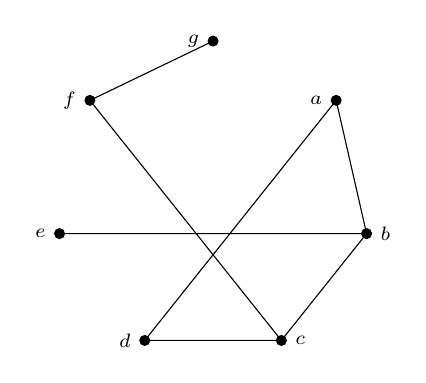
\begin{tikzpicture}
				\foreach \x in {1,...,7}{
				\coordinate (a\x) at (90-\x*360/7:2);
				}
				{\scriptsize
				\draw (a1) \vl{$a$} -- (a2) \vr{$b$} -- (a3) \vr{$c$} -- (a4) \vl{$d$} -- (a1) (a2) -- (a5) \vl{$e$} (a3) -- (a6) \vl{$f$} -- (a7) \vl{$g$};
				}
			\end{tikzpicture}
		\end{center}
	\end{solution}
	\vfill
	\part[8] One of the graphs below is isomorphic to $G$, the other is not.  Say which is which and then justify your answer by either specifying an isomorphism or explaining why no isomorphism can exist.
	{\scriptsize
	\begin{multicols}{2}
	\begin{center}
	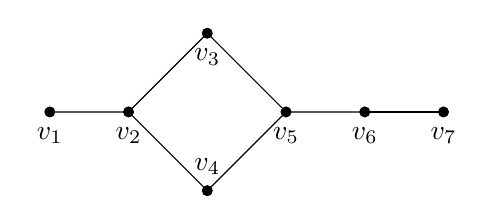
\begin{tikzpicture}
		\draw (180:2) \vb{$v_1$} -- (180:1) \vb{$v_2$} -- (90:1) \vb{$v_3$} -- (0:1) \vb{$v_5$} -- (0:2) \vb{$v_6$} (0:1) -- (-90:1) \va{$v_4$} -- (180:1);
		\draw (0:2) -- (0:3) \vb{$v_7$};
	\end{tikzpicture}

	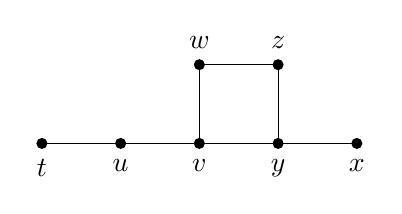
\begin{tikzpicture}
		\draw (3,0) \vb{$x$} -- (2,0) \vb{$y$} -- (2,1) \va{$z$} -- (1,1) \va{$w$} -- (1,0) \vb{$v$} -- (0,0) \vb{$u$} (1,0) -- (2,0);
		\draw (-1,0) \vb{$t$} -- (0,0);
	\end{tikzpicture}
\end{center}
\end{multicols}
	}
	\begin{solution}
		The graph on the left is not isomorphic to $G$.   We can see this because in $G$, there are two vertices of degree 3, and they are adjacent.  The graph of the left also has two vertices of degree 3, but they are not adjacent.  Thus there cannot be an isomorphism.

		The graph on the right is isomorphic to $G$.  Here is a function from $G$ to the graph on the left:
		\[\varphi = \twoline{a & b & c & d & e & f & g}{z & y & v & w & x & u & t}\]
		Note that $f$ must be sent to $u$ because these are the only vertices of degree 2 adjacent to a vertex of degree 1.  Then $g$ must be sent to $t$ and $c$ must be sent to $v$.  There is one vertex of degree 1 left ($e$) which must be sent to $x$.  Then continue.
	\end{solution}
	\vfill
	\vfill
\end{parts}




\newpage


\question I have a connected graph with five vertices of degree 7 and three vertices of degree 5.

\begin{parts}
	\part[4] How many edges does my graph have?  Briefly explain how you know, even though you haven't seen my graph.
	\begin{solution}
		The sum of the degrees will be $5 \cdot 7 + 3 \cdot 5 = 50$.  This is twice the number of edges, since we have counted each edge once on each of its ends.  So there are $e = 25$ edges.
	\end{solution}
	\vfill
	\part[6] Prove that my graph cannot possibly be planar.  Your proof should include full English sentences.
	\begin{solution}
		Suppose, for the sake of contradiction, that the graph was planar.  The graph has $v= 8$ vertices, and $e = 25$ edges.  Since the graph is planar, it satisfies Euler's formula, so we can compute $f = 2 +25 - 8 = 19$.  Each of these 19 faces would be bounded by at least three edges, although this counts the edges twice, so we also have
		\[3f \le 2e\]
		which says $57 \le 50$, a contradiction.  Therefore the graph cannot be planar.
	\end{solution}
	\vfill
	\vfill
\end{parts}





\end{questions}




\end{document}
